\begin{frame}{Exemple}
    \begin{center}
        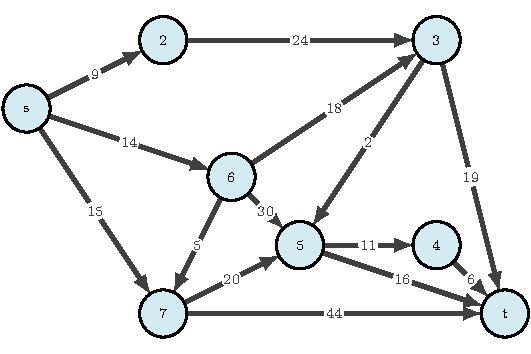
\includegraphics[height=.6\textheight]{fig/dijkstra-0.pdf}

    \end{center}
\end{frame}

\begin{frame}{Itérations de l'algorithme : traitement de $s$}
    \begin{center}
        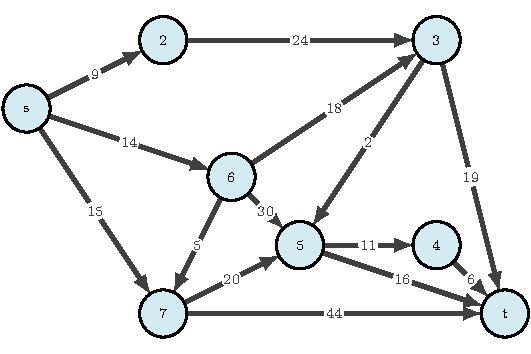
\includegraphics[height=.6\textheight]{fig/dijkstra-0.pdf}      
    \begin{tabular}{c|cccccccc}
      
        & \textbf{s}   &2      &7      &6      &5      &3      &4      &t      \\
        \hline
        \texttt{pred} & &s      &s      &s      &       &       &       &       \\
        \texttt{dist} & 0       &9      &15     &14     &inf    &inf    &inf    &inf    \\
            \end{tabular}
\end{center}
\end{frame}


\begin{frame}{Itérations de l'algorithme : traitement de $2$}
    \begin{center}
        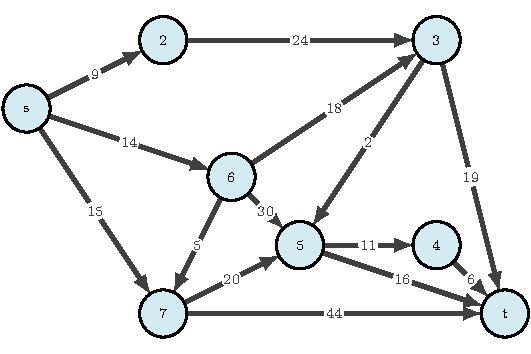
\includegraphics[height=.6\textheight]{fig/dijkstra-0.pdf}      
    \begin{tabular}{c|cccccccc}
      
        & \textbf{s}   &\textbf{2}     &7      &6      &5      &3      &4      &t      \\
        \hline
        \texttt{pred} & &s      &s      &s      &       &2      &       &       \\
        \texttt{dist} & 0       &9      &15     &14     &inf    &33     &inf    &inf    \\
                   \end{tabular}
\end{center}
\end{frame}

\begin{frame}{Itérations de l'algorithme : traitement de $6$}
    \begin{center}
        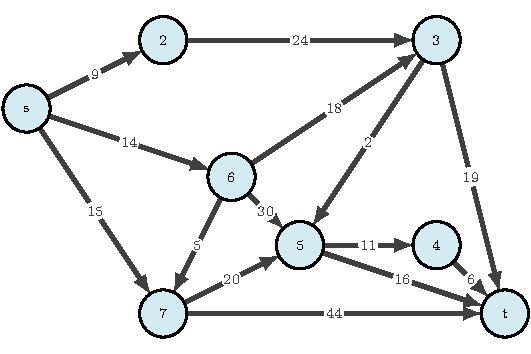
\includegraphics[height=.6\textheight]{fig/dijkstra-0.pdf}      
    \begin{tabular}{c|cccccccc}
      
        & \textbf{s}   &\textbf{2}     &7      &\textbf{6}     &5      &3      &4      &t      \\
        \hline
        \texttt{pred} & &s      &s      &s      &6      &6      &       &       \\
        \texttt{dist} & 0       &9      &15     &14     &44     &32     &inf    &inf    \\
                           \end{tabular}
\end{center}
\end{frame}


\begin{frame}{Itérations de l'algorithme : traitement de $7$}
    \begin{center}
        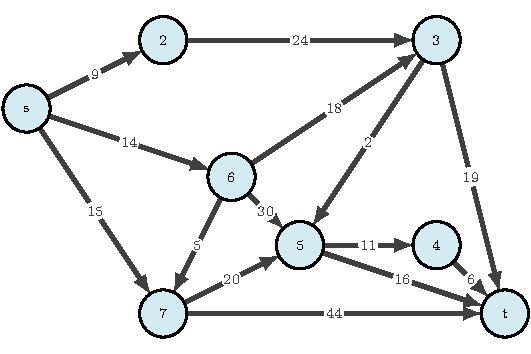
\includegraphics[height=.6\textheight]{fig/dijkstra-0.pdf}      
    \begin{tabular}{c|cccccccc}
      
        & \textbf{s}   &\textbf{2}     &\textbf{7}     &\textbf{6}     &5      &3      &4      &t      \\
        \hline
        \texttt{pred} & &s      &s      &s      &7      &6      &       &7      \\
        \texttt{dist} & 0       &9      &15     &14     &35     &32     &inf    &59     \\
    \end{tabular}
\end{center}
\end{frame}

\begin{frame}{Itérations de l'algorithme : traitement de $3$}
    \begin{center}
        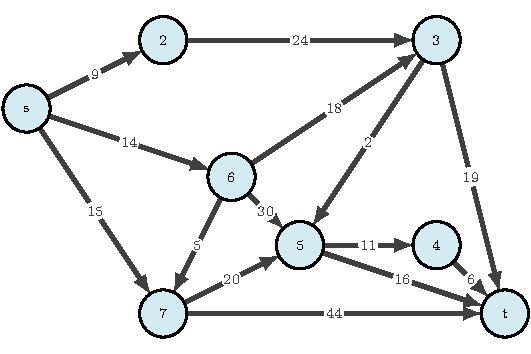
\includegraphics[height=.6\textheight]{fig/dijkstra-0.pdf}      
    \begin{tabular}{c|cccccccc}
      
        & \textbf{s}   &\textbf{2}     &\textbf{7}     &\textbf{6}     &5      &\textbf{3}     &4      &t      \\
        \hline
        \texttt{pred} & &s      &s      &s      &3      &6      &       &3      \\
        \texttt{dist} & 0       &9      &15     &14     &34     &32     &inf    &51     \\
    \end{tabular}
\end{center}
\end{frame}

\begin{frame}{Itérations de l'algorithme : traitement de $5$}
    \begin{center}
        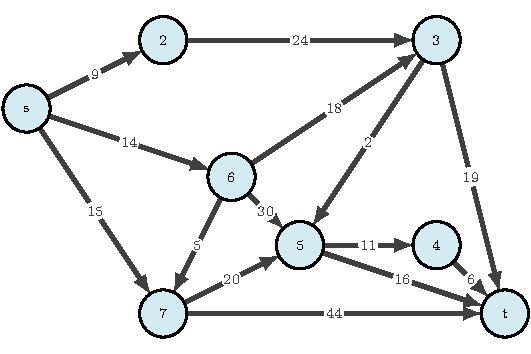
\includegraphics[height=.6\textheight]{fig/dijkstra-0.pdf}      
    \begin{tabular}{c|cccccccc}
      
        & \textbf{s}   &\textbf{2}     &\textbf{7}     &\textbf{6}     &\textbf{5}     &\textbf{3}     &4      &t      \\
        \hline
        \texttt{pred} & &s      &s      &s      &3      &6      &5      &5      \\
        \texttt{dist} & 0       &9      &15     &14     &34     &32     &45     &50     \\
            \end{tabular}
\end{center}
\end{frame}


\begin{frame}{Itérations de l'algorithme : traitement de $4$}
    \begin{center}
        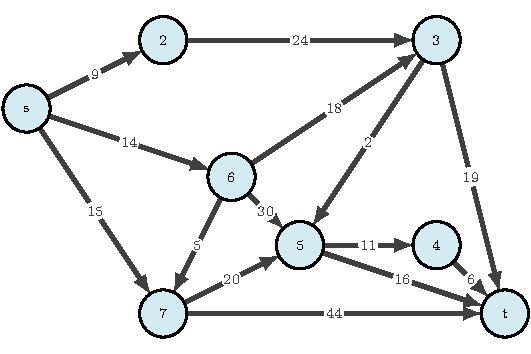
\includegraphics[height=.6\textheight]{fig/dijkstra-0.pdf}      
    \begin{tabular}{c|cccccccc}
      
        & \textbf{s}   &\textbf{2}     &\textbf{7}     &\textbf{6}     &\textbf{5}     &\textbf{3}     &\textbf{4}     &t      \\
        \hline
        \texttt{pred} & &s      &s      &s      &3      &6      &5      &5      \\
        \texttt{dist} & 0       &9      &15     &14     &34     &32     &45     &50     \\
                \end{tabular}
\end{center}
\end{frame}

\begin{frame}{Fin de l'algorithme}
    \begin{center}
        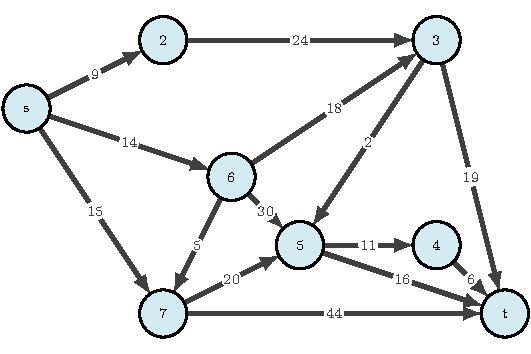
\includegraphics[height=.6\textheight]{fig/dijkstra-0.pdf}      
    \begin{tabular}{c|cccccccc}
      
        & \textbf{s}   &\textbf{2}     &\textbf{7}     &\textbf{6}     &\textbf{5}     &\textbf{3}     &\textbf{4}     &\textbf{t}     \\
        \hline
        \texttt{pred} & &s      &s      &s      &3      &6      &5      &5      \\
        \texttt{dist} & 0       &9      &15     &14     &34     &32     &45     &50     \\
                        \end{tabular}
\end{center}
\end{frame}




